\chapter{Experiment: hardware system}
In this chapter, we discuss experiments conducted on the hardware system. The content is organized into four sections. The first section provides an overview of the hardware setup for the double pendulum system. The second section delves into the system identification of the hardware. The third section details our approach to addressing the sim-to-real gap challenge. The final section presents the successful outcomes of our hardware experiments.

\section{Hardware setup}
Mechanically, the double pendulum system is a straightforward 2-R linkage. The first revolute joint attaches to the base, while the second one connects the two links. Quasi-direct drive motors are mounted on each joint to provide torque, and a counterweight is positioned at the end of the second link.

Our mechanical design for the double pendulum underwent two iterations. In the initial design, the base consisted of a bent aluminum plate, and the links featured a sandwich structure with aluminum on the outside and engineering plastic on the inside. These links were of homogeneous size, meaning that the cross-sectional areas at the link intersections were consistent. We abandoned this design due to rotational imbalances. Specifically, the rotation plane of the links wasn't consistently perpendicular to the motor axes, leading to vibrations and accelerated wear during regular use. In extreme cases, when the links rotated at high angular velocities, this imbalance was exacerbated. This not only resulted in the links bending but also led to catastrophic system failures. Such failures presented significant safety risks to personnel.

In the second iteration, we addressed the issues encountered in the previous design, leading to two major modifications. First, we replaced the aluminum-plastic combination with a carbon fiber-foam blend. While the incorporation of carbon fiber marginally increased the cost, it significantly boosted the yield strength. Second, we introduced triangular-shaped links with central cutouts. This design, while lightweight, also substantially enhanced the yield strength due to the changed intersections. Overall, this iteration resulted in a mechanical structure that is considerably more reliable than the first.

\begin{figure}[H]
    \centering
    \begin{subfigure}[b]{0.3\textwidth}
        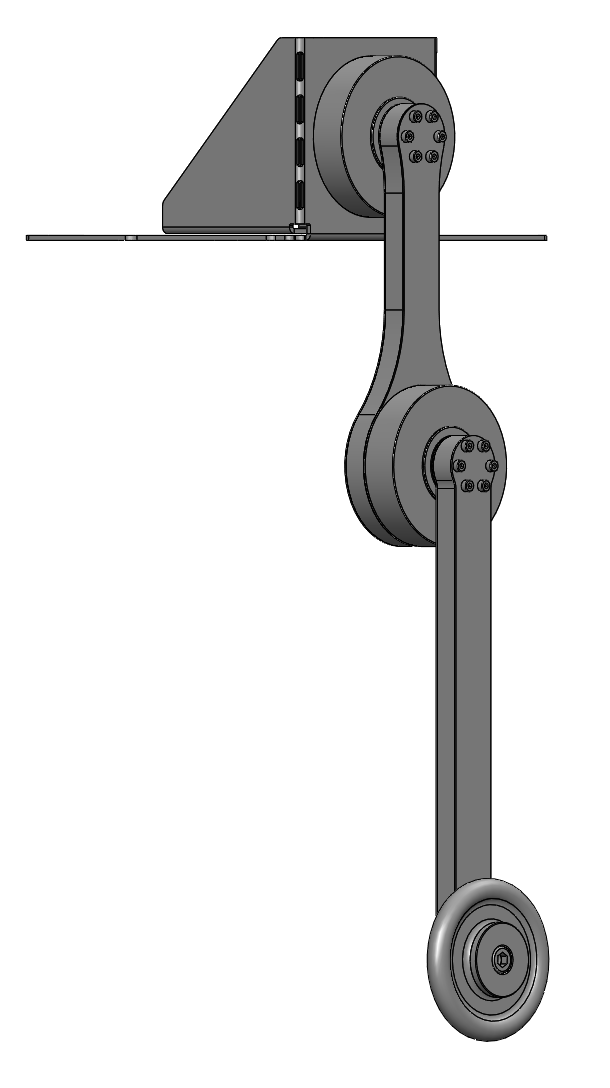
\includegraphics[width=\textwidth]{figures/hardware_setup/double_pendulum_it1_v1.png}
        \caption{Iteration 1 in isometric view}
        \label{fig:image1}
    \end{subfigure}
    \hfill
    \begin{subfigure}[b]{0.3\textwidth}
        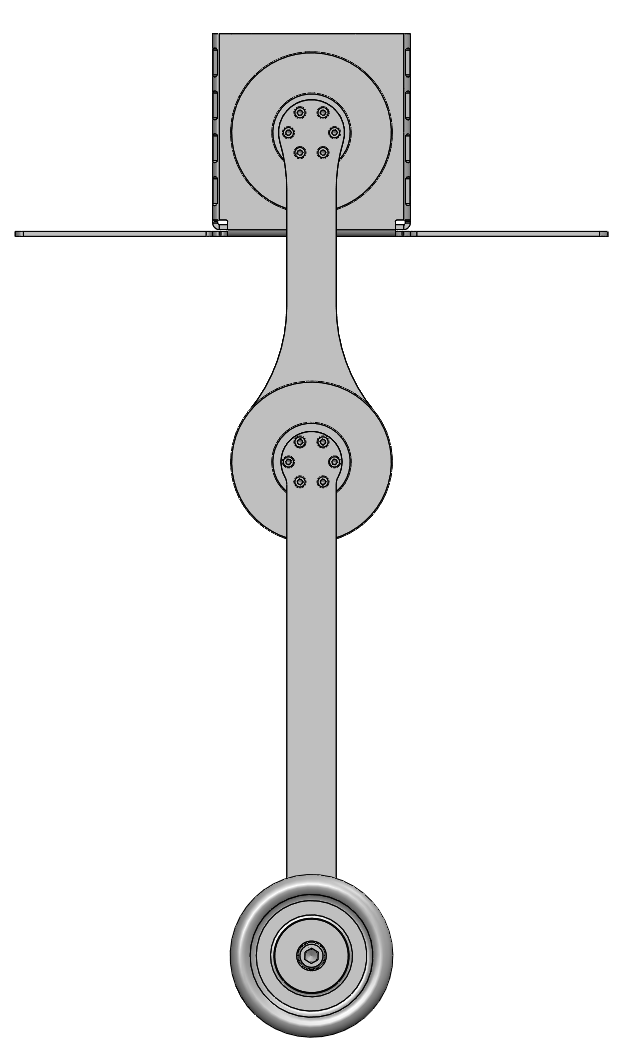
\includegraphics[width=\textwidth]{figures/hardware_setup/double_pendulum_it1_v2.png}
        \caption{Iteration 1 in front view}
        \label{fig:image2}
    \end{subfigure}

    \vspace{1em} % or use \bigskip or \medskip depending on the space you want

    \begin{subfigure}[b]{0.3\textwidth}
        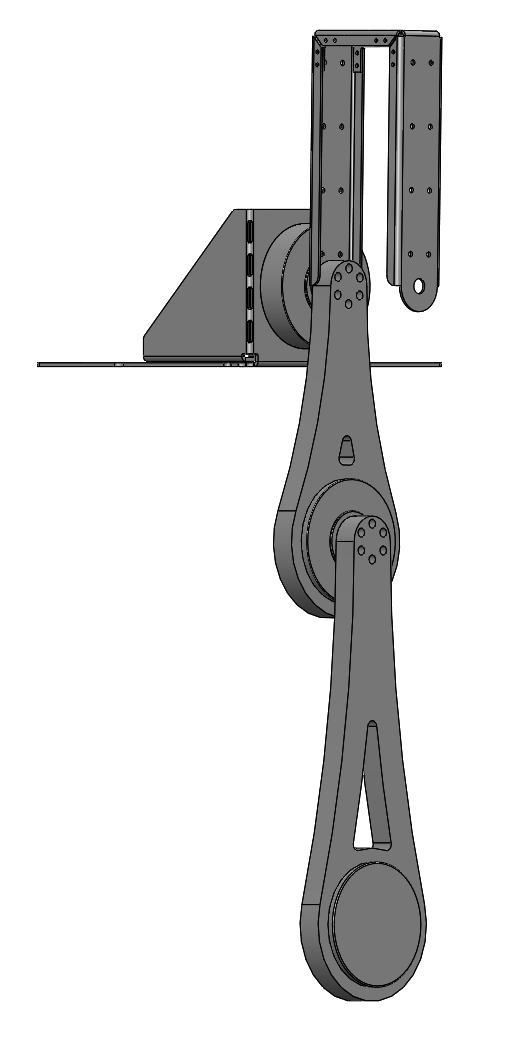
\includegraphics[width=\textwidth]{figures/hardware_setup/double_pendulum_it2_v1.png}
        \caption{Iteration 2 in isometric view}
        \label{fig:image3}
    \end{subfigure}
    \hfill
    \begin{subfigure}[b]{0.3\textwidth}
        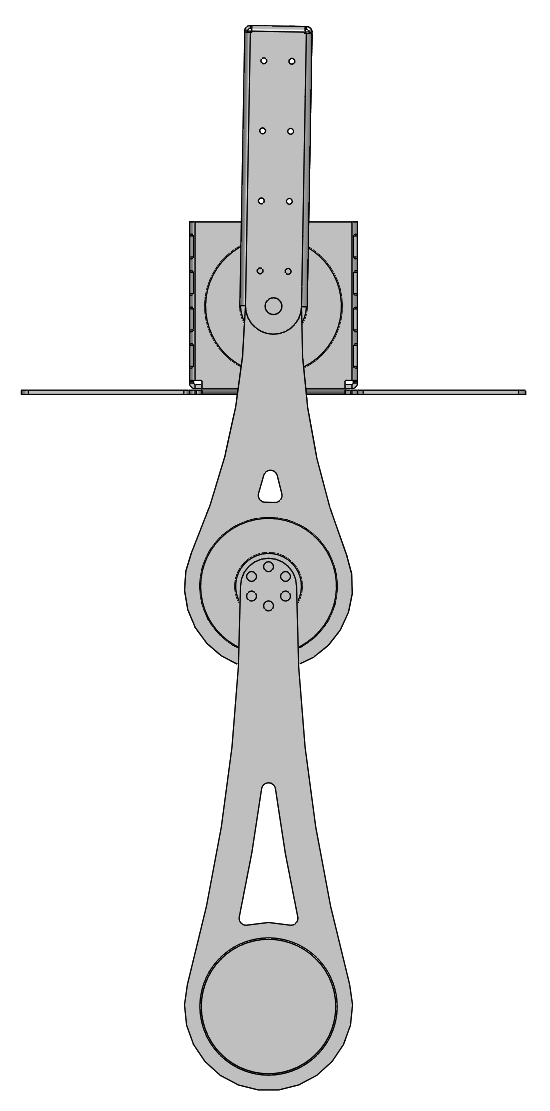
\includegraphics[width=\textwidth]{figures/hardware_setup/double_pendulum_it2_v2.png}
        \caption{Iteration 2 in front view}
        \label{fig:image4}
    \end{subfigure}
    \caption{Double pendulum mechanical system iteration 1 and iteration 2}
    \label{fig:four_images}
\end{figure}

For the quasi-direct drive(QDD) motors, we selected the AK80-6 V100 motors from the company CubeMars. This motor's design facilitates easy mounting from both the front and rear ends. As depicted in Figure5.2(b), the motor's maximum torque during continuous operation is 6 Nm, which aligns well with our torque limit of 5 Nm. Additionally, the motor is designed for compatibility with both serial bus and CAN bus, simplifying the development process.


\begin{figure}[htbp]
  \centering
  \begin{subfigure}[b]{0.45\textwidth}
    \centering
    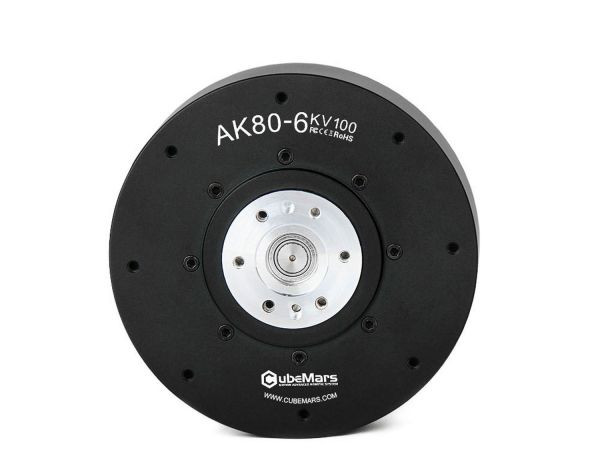
\includegraphics[width=\textwidth]{figures/hardware_setup/motor.jpg}
    \caption{AK80-6 V100 motor}
    \label{fig:subfiga}
  \end{subfigure}
  \hfill
  \begin{subfigure}[b]{0.45\textwidth}
    \centering
    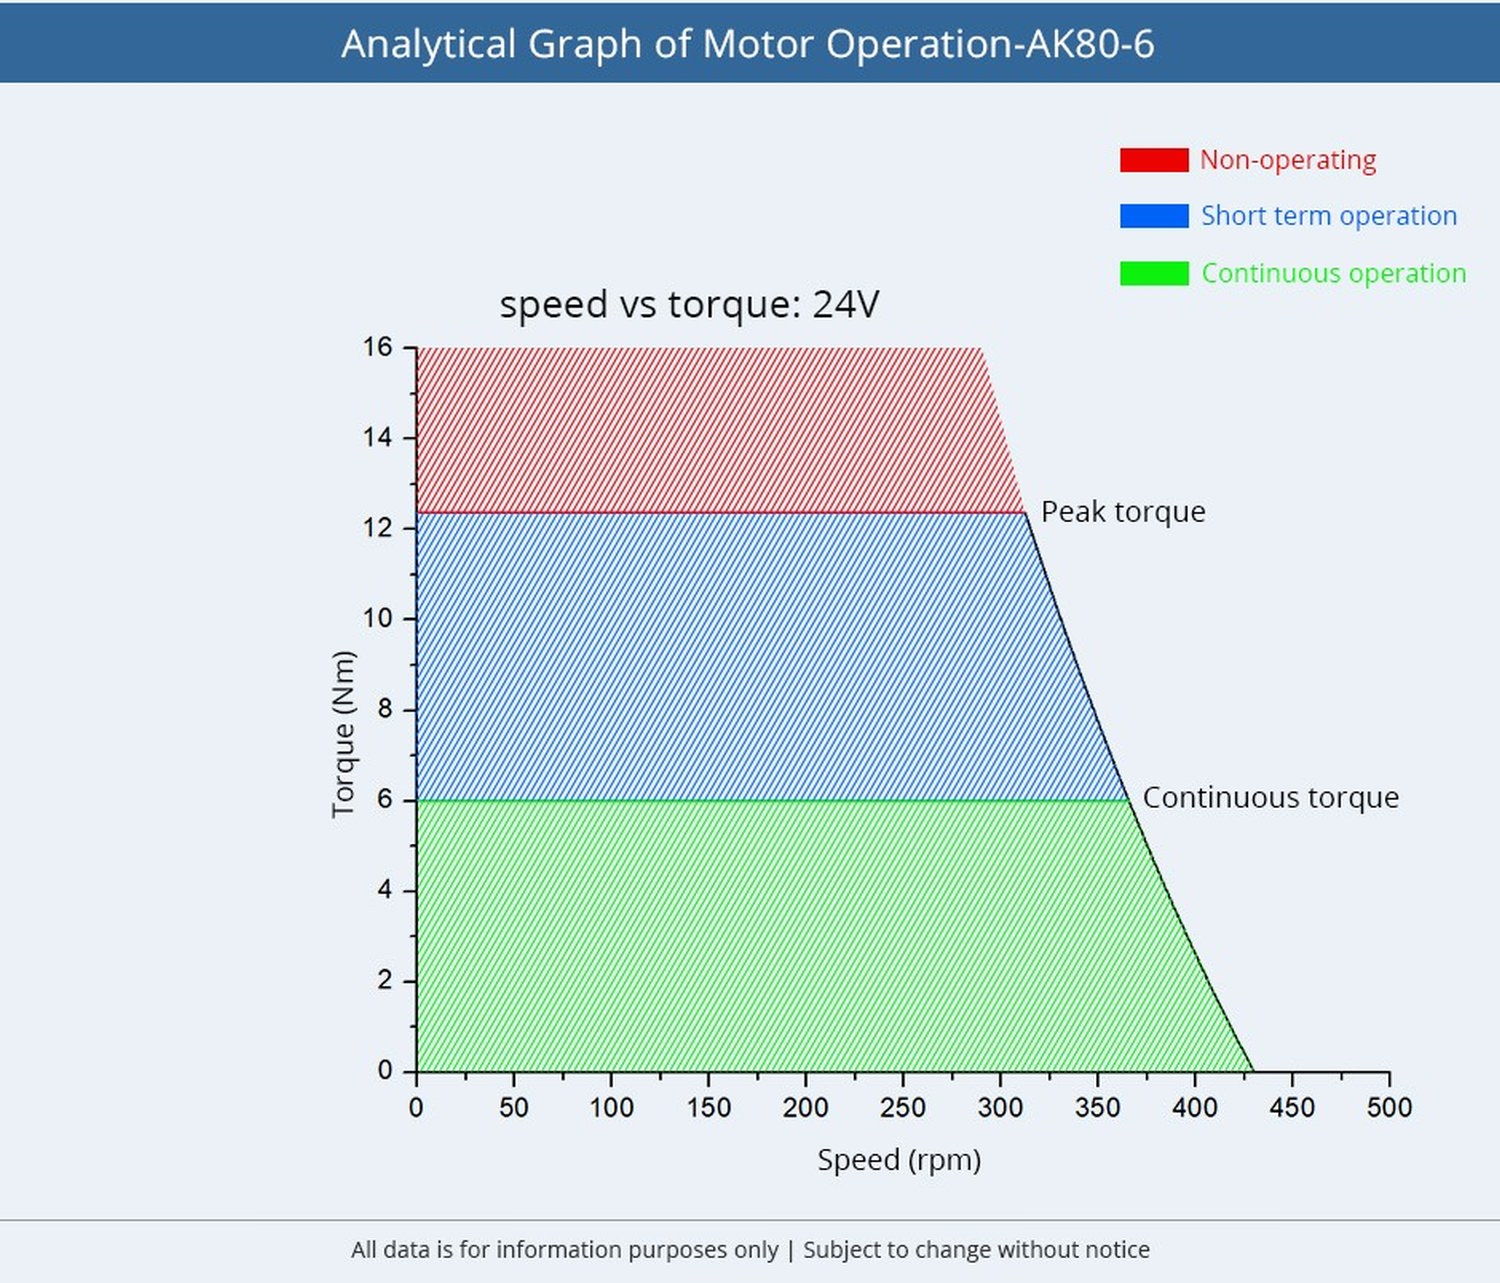
\includegraphics[width=\textwidth]{figures/hardware_setup/torque_speed_curve.jpg}
    \label{fig:subfigb}
    \caption{Speed-torque diagramm}
  \end{subfigure}
  \caption{Quasi direct drive motor AK80-6 V100}
  \label{fig:twosubfigures}
\end{figure}

For communication, We have chosen CAN in this implementation. The Controller Area Network (CAN) bus is a robust, flexible, and efficient communication protocol that has been employed in various applications. There are many advantages to using the CAN bus for control. The CAN bus provides error checking and fault confinement capabilities. It operates in real-time, enabling high control frequencies with relatively simple wiring. In our configuration, there is only one master node (the PC) and two slave nodes (two motors). The control loop simply consists of a CAN-to-USB converter, one CAN high cable, and one CAN low cable, with a termination resistor of \(120 \Omega\) at both ends. The detailed connection is depicted in the figure below:

\begin{figure}[H]
    \centering
    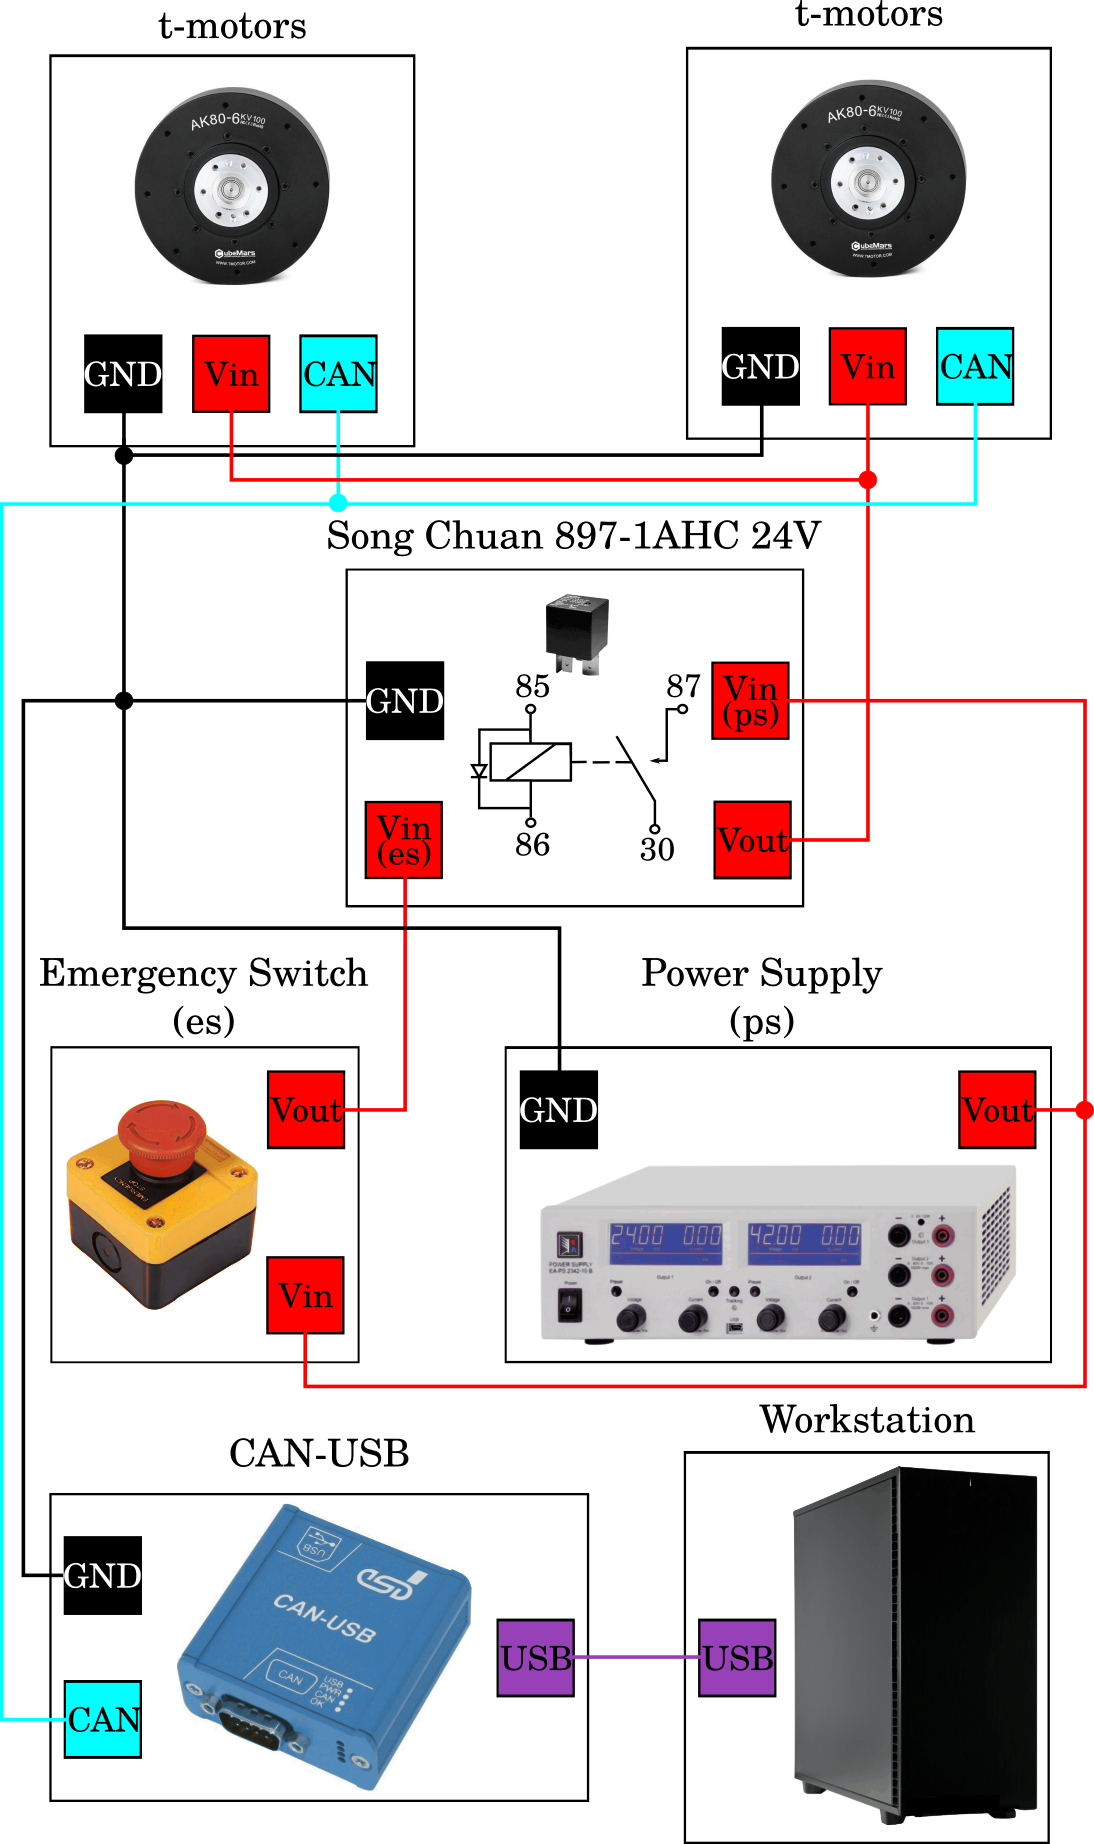
\includegraphics[width=0.7\linewidth]{figures/hardware_setup/wiring-diagram.png}
    \caption{Wiring diagram}
    \label{fig:my_label}
\end{figure}

To ensure a higher control frequency of around 500 Hz, we chose the CAN-USB/2 product from ESD GmbH Hannover. This specialized CAN-to-USB interface utilizes USB 2.0, which supports a data rate of 480 Mbit/s. Its CAN capability is 1 Mbit/s, in accordance with ISO 11898-2. Additionally, it supports the SocketCAN interface included in the Linux Kernel 2.6, making it easier to use in a Linux development environment.

\begin{figure}[H]
    \centering
    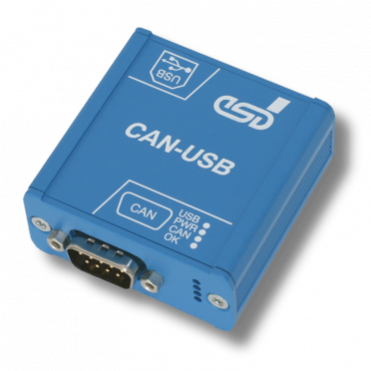
\includegraphics[width=0.3\linewidth]{figures/hardware_setup/can_blue_box.png}
    \caption{High speed CAN to USB interface[not the same version, correct it]}
    \label{fig:my_label}
\end{figure}

Due to accidents that occurred during testing with the mechanical systems from the first iteration, several safety protocols have been implemented to ensure the safety of both human lives and equipment. Four major measures have been taken.

An emergency stop is connected directly to the 24V power source. If the behavior of the double pendulum deviates from the expected range during testing, the power supply can be manually cut off immediately. The energy in the mechanical system will dissipate rapidly, and the system will return to its initial state automatically.

In scenarios where the system is moving at a very high speed when the emergency stop is engaged, the motors attached to the revolute joints act as generators, dissipating the mechanical energy from the system's motion. The generated current is fed back into the circuit, and in extreme cases, it could overload the power supply. To counteract this, a capacitor is connected to the power supply to absorb any electrical surge resulting from a sudden stop.

\begin{figure}[htbp]
    \centering
    \includegraphics[width=0.4\textwidth]{example-image}
    \caption{picture of the capacitor}
    \label{fig:example_figure}
\end{figure}

Further, speed and position limits have been set at the software level. As the links of the pendulum can experience vibrations and rotational imbalances at high speeds, potentially leading to structural disassembly, a speed limit of 20 rad/s has been established. Any speed exceeding this value will trigger a full system stop, equivalent to pressing the emergency stop button. The position limit is set to \(2\pi\) for both pos1 and pos2. Excessive rotations could cause the CAN and power cables to become entangled, leading to interference and potential cable damage.

Lastly, to guard against unpredictable system failures, a custom protective cage has been constructed using aluminum profiles and thick acrylic boards. This cage fully encloses the double pendulum hardware, significantly reducing the risk of accidents.

These measures have been instrumental in minimizing potential hazards during testing and operation.

\begin{figure}[htbp]
    \centering
    \includegraphics[width=0.6\textwidth]{example-image}
    \caption{a overview of experiment setup}
    \label{fig:example_figure}
\end{figure}

\section{System identification}
System identification is the process of deriving mathematical models of dynamic systems from observed input-output data. This method is fundamental in control theory, used to analyze, predict, and control the behavior of real-world systems. After setting up the hardware system and before transitioning the working model from a successful simulation to the real system, it's necessary to undergo a system identification process. This helps ascertain the real-world parameters governing the dynamics of the double pendulum.

Out of all model parameters, 15 are selected. While the naturally provided parameters \(g\) and \(g_r\) are held constant, the easily measurable parameters \(l_1\) and \(l_2\) are considered independent. The remaining system parameters, which are 
\[
m_1 r_1,\, m_2 r_2,\, m_1,\, m_2,\, I_1,\, I_2,\, I_r,\, b_1,\, b_2,\, c_{f1},\,c_{f2}
\]

need to be identified. The ultimate objective is to discern the parameters of the dynamic matrices present in the equations of motion.
\begin{equation}
M \ddot{q} + C(q, \dot{q}) \dot{q} - G(q) + F(\dot{q}) - D u = 0
\end{equation}

By running excitation trajectories on the actual hardware, data tuples in the form \((q, \dot{q}, \ddot{q}, u)\) can be collected. To determine the most accurate system parameters, one can leverage the linearity of the dynamic matrices \(M\), \(C\), \(G\), and \(F\) in relation to the independent model parameters. Consequently, a least squares optimization can be performed on the recorded data, relative to the dynamics equation.

The identified model parameters are shown in table below:

\begin{table}[H]
\centering
\begin{tabular}{|c|c|}
\hline
\textbf{Parameter} & \textbf{Value} \\
\hline
$I_1$ & 0.031887199591513114 \\
$I_2$ & 0.05086984812807257 \\
$I_r$ & 6.287203962819607e-05 \\
$b_1$ & 0.001 \\
$b_2$ & 0.001 \\
$c_{f1}$ & 0.16 \\
$c_{f2}$ & 0.12 \\
$g$ & 9.81 \\
$g_r$ & 6.0 \\
$l_1$ & 0.2 \\
$l_2$ & 0.3 \\
$m_1$ & 0.5234602302310271 \\
$m_2$ & 0.6255677234174437 \\
$r_1$ & 0.2 \\
$r_2$ & 0.25569305436052964 \\
\hline
\end{tabular}
\caption{Parameter values from system identification}
\label{tab:parameters}
\end{table}


\section{Sim2Real problem}
Transferring working models from simulation to real systems to produce similar performance has always been a challenge in controller design. This challenge is even more pronounced in model-free reinforcement learning for several reasons.

Firstly, model-free reinforcement learning relies solely on interaction with the environment to gain experience and select actions. While a simulation environment is merely a simplification of the real-world scenario, the agent in simulation might not capture all the factors, such as friction, sensor noise, or real-world dynamics, accurately. Therefore, a control policy optimized for a simplified model might not perform as expected in the more intricate real world.

Secondly, many simulations operate in discrete time and space, whereas the real world functions continuously. In our implementation, the control frequency presents a significant challenge. We use a control frequency of 100 Hz in simulation; however, it does not suffice in the real system. To enhance performance, we increased the control frequency to 400 Hz when experimenting on the real system, and this adjustment yielded positive results.

Thirdly, uncertainties in the environment can lead to substantial complications when attempting to apply learned strategies or actions. Generally speaking, the uncertainty of the environment is addressed by the robustness of the model. However, for highly chaotic systems like the pendubot or acrobot, even slight measurement errors can result in significant deviations from the planned behavior. Our model for controlling the pendubot and acrobot requires a higher level of robustness or a more effective sim2real transfer method.

\subsection{Validation with noisy simulation}
Our approach to addressing the sim2real challenge involves training multiple agents using the SAC algorithm under similar setups. Subsequently, we validate them in a noisy simulation. Only those agents that prove robust against perturbations in this noisy environment proceed to real system testing. Any agent failing these noisy simulation tests is deemed insufficiently robust and is discarded.

Throughout our experiments with real systems, we identified four critical factors contributing to successful swing-up and stabilization. Of these, friction emerged as the most significant. This is because our agent training was conducted in an ideal environment devoid of friction, thereby making friction the primary differentiator between the simulation and real-world conditions. To counter this, we adopted a friction compensation approach, beginning with modeling based on Coulomb's friction.

Coulomb's friction model is among the simplest existing friction models. It possesses two primary advantages: it's independent of both the contact area and the relative velocity. The frictional force (\( F_f \)) is directly proportional to the normal force (\( F_n \)) between the surfaces, represented by:
\begin{equation}
F_{fi} = c_{fi} \arctan(100\dot{q_i})\, , \quad i = 1,2
\end{equation}

where \( c_f \) is the coefficient of kinetic friction. This frictional force opposes the relative motion between the surfaces. To neutralize this force, friction compensation applies torque in the same direction as the angular motion, energizing the system to mitigate friction's effects.

Though friction coefficients \( c_{f1} \) and \( c_{f2} \) were determined during the system identification phase, they seemed imprecise during real system tests. Consequently, we resorted to free fall tests to estimate the coefficients, fine-tuning them manually until the system behaved conservatively under friction's influence.

The second most critical factor is measurement noise. While the AK80-6 motors use built-in encoders to measure the position difference from the initial position with high accuracy, velocity measurement, which is derived from the first derivative of the position measurement, tends to have a relatively high error. In the simulation environment, we assume zero measurement error. However, in real-world applications, this error becomes significant.

To address this issue, we model the measurement error as a normal distribution where the mean corresponds to the true velocity value and the standard deviation is manually adjustable. Let's consider the measurement noise vector \(\boldsymbol{\epsilon} = 
\begin{bmatrix}
\delta\text{pos1},
\delta\text{pos2},
\delta\text{vel1},
\delta\text{vel2}
\end{bmatrix}^T\). We model this noise as following a multivariate normal distribution, given by:
\begin{equation}
\boldsymbol{\epsilon} \sim \mathcal{N}(\boldsymbol{\mu}, \boldsymbol{\Sigma})
\end{equation}

where \(\boldsymbol{\mu}\) is the mean vector (which represents the true values in the absence of noise), and \(\boldsymbol{\Sigma}\) is the \(4 \times 4\) covariance matrix that captures the spread or uncertainty of the noise in each dimension. Since the measurements of the four states are considered independent of each other, \(\boldsymbol{\Sigma}\) is diagonal.

Latency is the third significant factor. Since any communication system requires time to transmit and receive data, and programs also take time to execute, latency is inevitable. This latency poses a substantial risk to control systems, especially those based on reinforcement learning. This is because reinforcement learning is grounded in the principles of Markov Decision Processes (MDPs) which adhere to the Markov property. This property dictates that the future state of a process is contingent only on the current state and action, not on the sequence of states that led to it. Latency undermines the Markov property by causing state mismatches and creating dependencies on historical data. If not addressed, this can have severe consequences.

The fourth factor to consider is torque responsiveness. We observed that when confronted with rapidly alternating control signals with significant differences between time steps, the motor struggles to produce torque that matches the control signal. In other words, the motor cannot respond timely to changes in torque. This lag means that the controller cannot operate at its full potential due to hardware constraints. Some potential solutions to this include reducing the control frequency and increasing torque smoothness.

In summary, we take into account friction, measurement error, latency, and torque responsiveness in the noisy simulation to select the most suitable agent.

As shown in the figure below, a trained pendubot agent successfully executed a swing-up and stabilization in the noisy simulation environment, indicating its robustness is sufficient for real-world application.

\begin{figure}[htbp]
    \centering
    \fbox{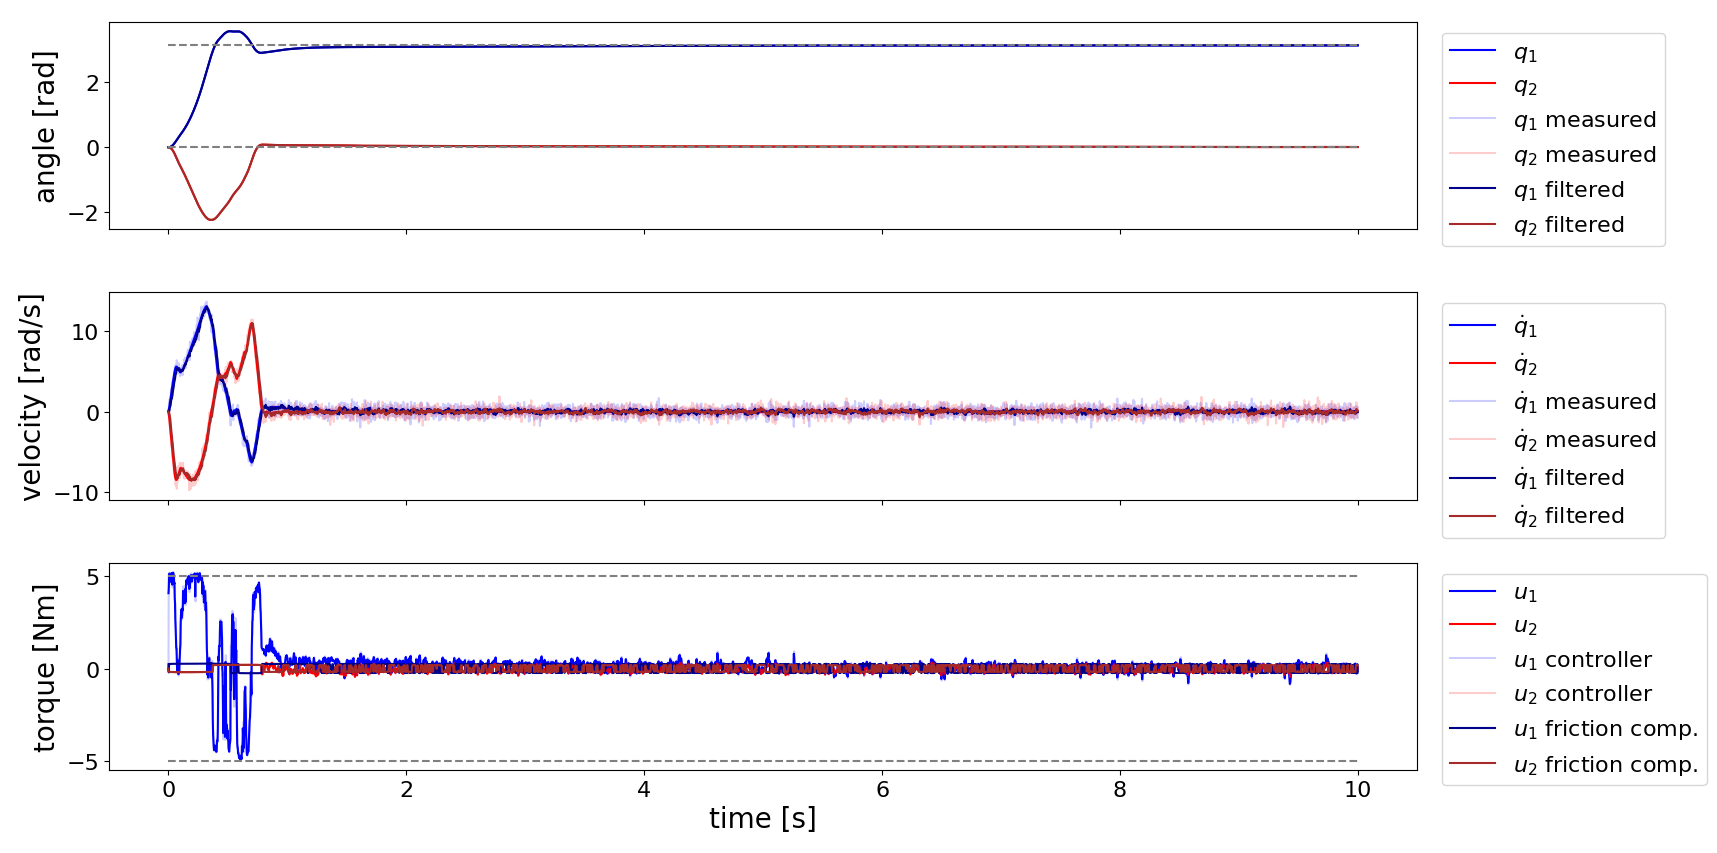
\includegraphics[width=0.9\textwidth]{figures/hardware_result/pendubot_noisy_unclipped.png}} % Second image
    \caption{pendubot noisy simulation result}
    \label{fig:image_b}
\end{figure}

\subsection{Training with domain randomization}
Domain randomization[some paper] is a classic technique used to bridge the gap between simulation and reality. Its primary goal is to allow a model, when generalized in a simulated environment, to perform effectively in real-world scenarios without needing labeled real-world training data.

The concept of domain randomization originates from the field of computer vision. Instead of training a model in a single, fixed simulation, the model is exposed to a more varied and noisy environment by introducing random variations to the ideal simulation. Techniques commonly employed in vision-based systems include changing the colors and textures of objects, modifying the lighting conditions, adjusting object shapes and sizes, introducing random noise to sensor data, and perturbing physical properties like friction or mass.

In our effort to apply domain randomization to robotic manipulation tasks, we opted to introduce random measurement noise to both position and velocity and to introduce perturbations to model parameters. These perturbations are considered independent of one another and follow a normal distribution. The mean of this distribution is the true value, and there's a tunable standard deviation.

[results and more explanation]

\section{Real hardware results}
In this section, we present the results from the real hardware tests. Only agents trained for the pendubot setup successfully passed the noisy simulation check, so results are limited to this setup. 

\begin{figure}[H]
    \centering
    \includegraphics[width=0.45\textwidth]{figures/double_pendulum_real_system.png}
    \caption{Double pendulum in real system}
    \label{fig:image_b}
\end{figure}

The complete real-world test procedure is as follows: power up, manually set the initial state, release the emergency button, run the initialization script (which enables the motor, sets the current position to zero, and tests the CAN connection), confirm the start of the test, record video, draw plots, and exit the test. This procedure is illustrated in the flow chart below:

\begin{figure}[H]
    \centering
    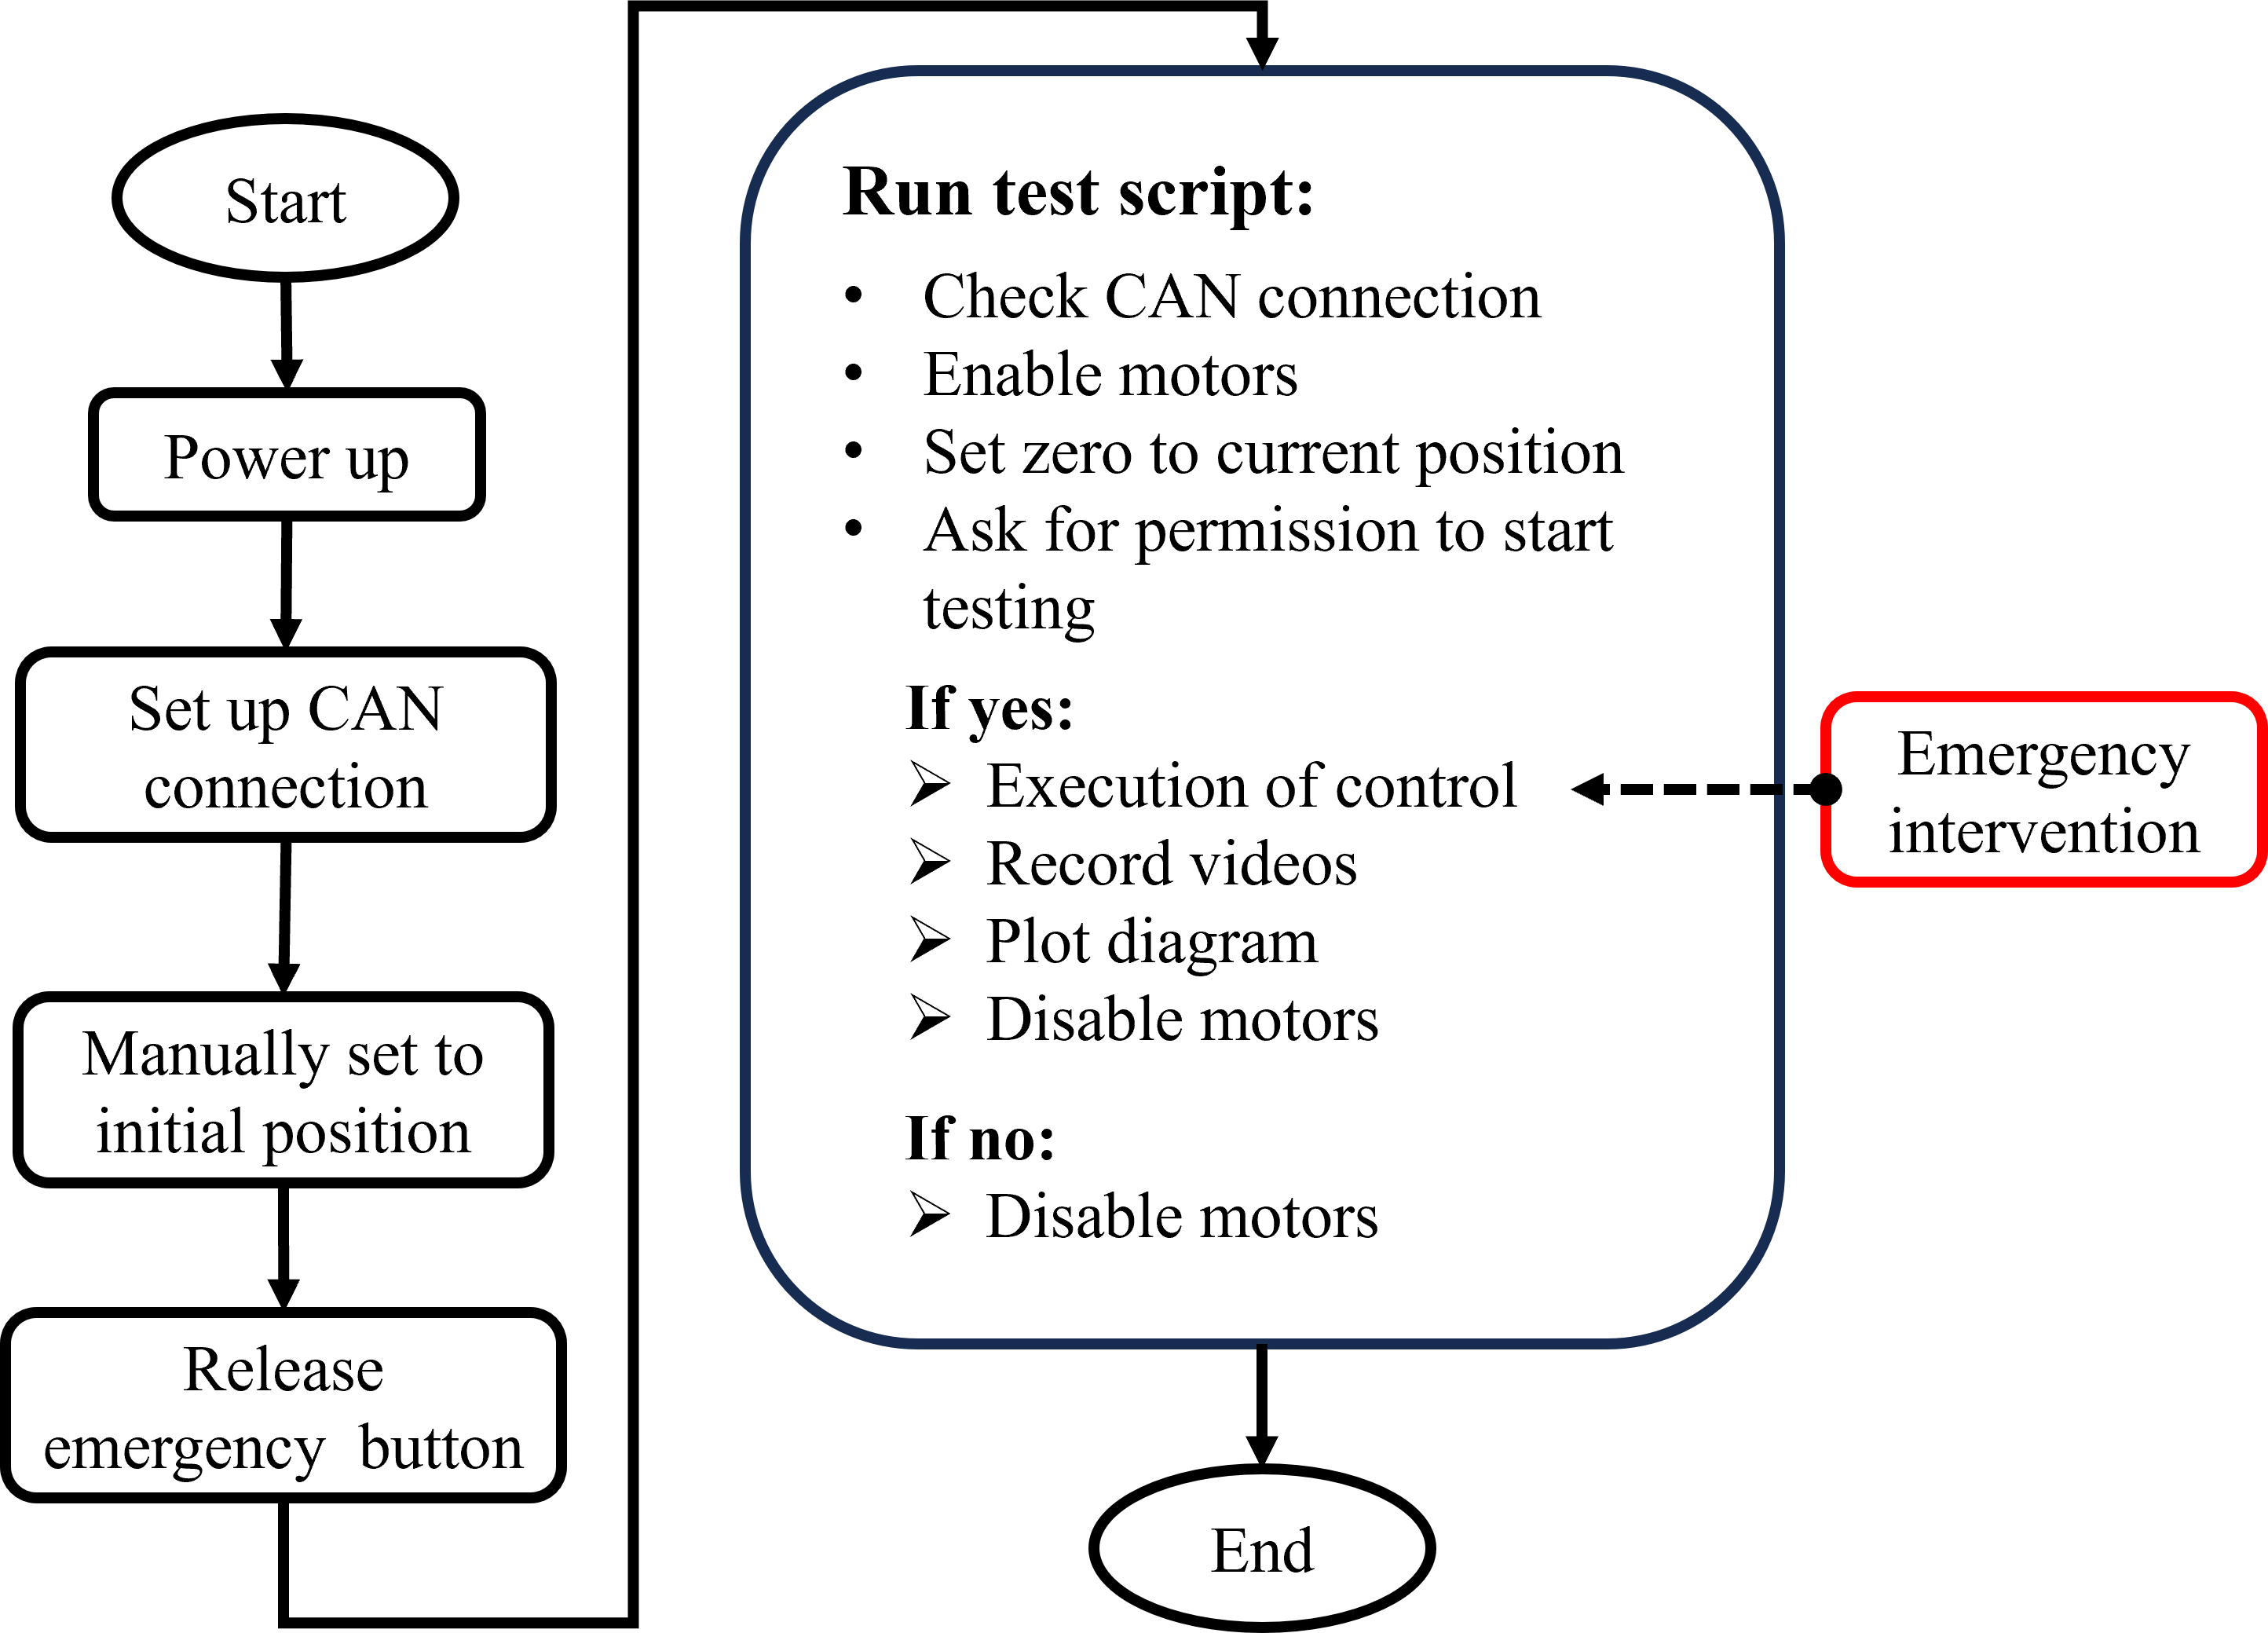
\includegraphics[width=0.9\textwidth]{figures/hardware_setup/testing_procedure.png}% Second image
    \caption{Real hardware system testing procedure}
    \label{fig:image_b}
\end{figure}
A remote testing system has been established to allow global access and sharing of our double pendulum testing hardware. This infrastructure was developed for the IJCAI 2023 competition, RealAIGym. Several groups have tested their algorithms on this remote system, including teams from the University of Padova and the Technical University of Darmstadt.

\subsection{Pendubot results}
Below is an example of one of our successful tests. [some explanation] We executed a sequence of 10 tests to determine the success rate and other key metrics for evaluating performance and robustness. These results will be discussed in the next chapter. 

\begin{figure}[H]
    \centering
    \includegraphics[width=0.7\linewidth]{example-image}
    \caption{Pendubot results on real systems}
    \label{fig:my_label}
\end{figure}

\subsection{acrobot results}
acrobot:

\cleardoublepage
